% !TEX encoding = UTF-8 Unicode
\documentclass[12pt, oneside]{article}  
\usepackage[T1]{fontenc}
\usepackage[utf8]{inputenc}
\usepackage[czech]{babel}					
\usepackage{amsmath}
\usepackage{amssymb}
\usepackage{graphics}
\usepackage{listings} 
\usepackage{graphicx}
\usepackage{forest}
\usepackage{fullpage}
\usepackage{cancel}
\usepackage{subfiles}
\usepackage{hyperref}
\title{\vspace{-12ex}Swarm - dokumentace}
\author{\vspace{-10ex}Tomáš Karella}
\date{}
\begin{document}
	\maketitle
\clearpage
\tableofcontents
\clearpage
\section{Úvod}
Cílem Swarm programu bylo implementovat framework pro evoluci robotického swarmu, jenž umožňuje variabilní tvorbu map, robotů a ostatních entit prostředí( paliva, interaktivních překážek...). Na základě vytvořeného prostředí spustí simulaci akcí jednotlivých robotů a ohodnocuje jejich chování. Poskytuje negrafickou multithread simulaci a vizuální vezi pro sledování korektosti simulace a vyvinutého chování. 
\subsection{SwarmSimFramework} 
Vlastní framework, definice rozhraní, vlastní kód simulace, příklady scénářů
\subsection{Další části:}
\begin{itemize}
	\item SwarmSimVisu - 
	Visualizace průběhu simulace, prohlížení vygenerovaných chování. 
	\item Intersection2D - 
	Implementace jednoduchých průsečíků v 2D prostoru (přímky, úsečky, kružnice).
\end{itemize}
\clearpage
\section{Uživatelská dokumentace}
\section{Požadavky}
Aplikace podporuje operační systém Windows. Pro její spuštění je potřeba mít nainstalovaný .NET Framework alespoň verze 4.7. Instalace verze 4.7 se nachází ve složce \textbf{\textbackslash bin\textbackslash dep}.  
\subsection{Spuštění}
Spuštění hlavni konzolové aplikace je možné pouze s následujícími parametry: \par
\begin{itemize}
\item \textit{-de konfigurační\_soubor.expe} - spustí diferenciální evoluci s danou konfigurací \begin{itemize}
	\item bez dalších parametrů vygeneruje první generaci náhodně
	\item očekává jména souboru s serializovanou první generací, za každého robota jeden soubor 
	\end{itemize}
\item \textit{-es konfigurační\_soubor.es} - spustí evoluční strategie s danou konfigurací 
\begin{itemize}
	\item první generace jsou nastaveny v konfiguračním souboru
\end{itemize}
\item \textit{-stats nastavení\_mapy.stats} - spustí 100 simulací a na standartní výstup vypíše průměrné charakteristiky mapy  
\end{itemize} 
\subsection{Výstupy:}
Výstupy evolučních algoritmů se kvůli paralelizaci liší.
\subsubsection*{-de}
V místě běhu si program vytvoří pracovní složku (její název je uveden v konfiguračním souboru) a po skončení optimalizace přidá do místa běhu serializovanou poslední populaci, kdy se vygeneruje pro každý druh robota jeden soubor \textit{jméno\_experimentuBrain[pořadí robota].json}. 
\par 
Pracovní složka obsahuje soubory s serializovanými nejlepšími jedincemi, soubory mají název \textit{[číslo\_generace]bestbrain[pořadí\_robota].json}. Dále soubor s výpisem fitness pro vytváření grafů, každý řádek má podobu \textit{[číslo\_generace];fitness}
\par 
Na standartní výstup jsou vypisovány průběžné statistiky fitness, očekávaný čas ukončení, apod.
\subsubsection*{-es}
Také v místě běhu vytvoří pracovní složku s názvem dle konfiguračního souboru. Ovšem jejich struktura je odlišná, protože každý jedinec běží v jiném vlákně. Každý jedinec má v pracovní složce svou vlastní složku s číslem vlákna a soubor s výpisem fitness pro graf ve stejném formátu jako u -de.
\par
Jednotlivé podsložky, pak obsahují serializovaného jedince z každé generace a 20 nejlepších jedinců. Nejlepší jedinci pak mají název \textit{best[pořadí\_robota]-název\_robota} a chování z generací \textit{[číslo\_generace]-název\_robota}. 
\par 
Na standartní výstup jsou vypisovány průběžné informace o aktuální populaci a číslu iterace jednotlivých vláken. 
\subsubsection*{-stats}
Vypisuje pouze na standartní výstup průměrné charakteristiky ze 100 simulací daných konfiguračním souborem. Každý řádek pak odpovídá jedné charakteristice a za \textbf{:} je uvedena jejich hodnota.  \clearpage
\subsection{GUI}
Program poskytující vizualizaci chování jednotlivých robotů se jmenuje \textit{SwarmSimVisu}. Po jeho spuštění se objeví úvodní okno.
\begin{figure}[h]\centering
		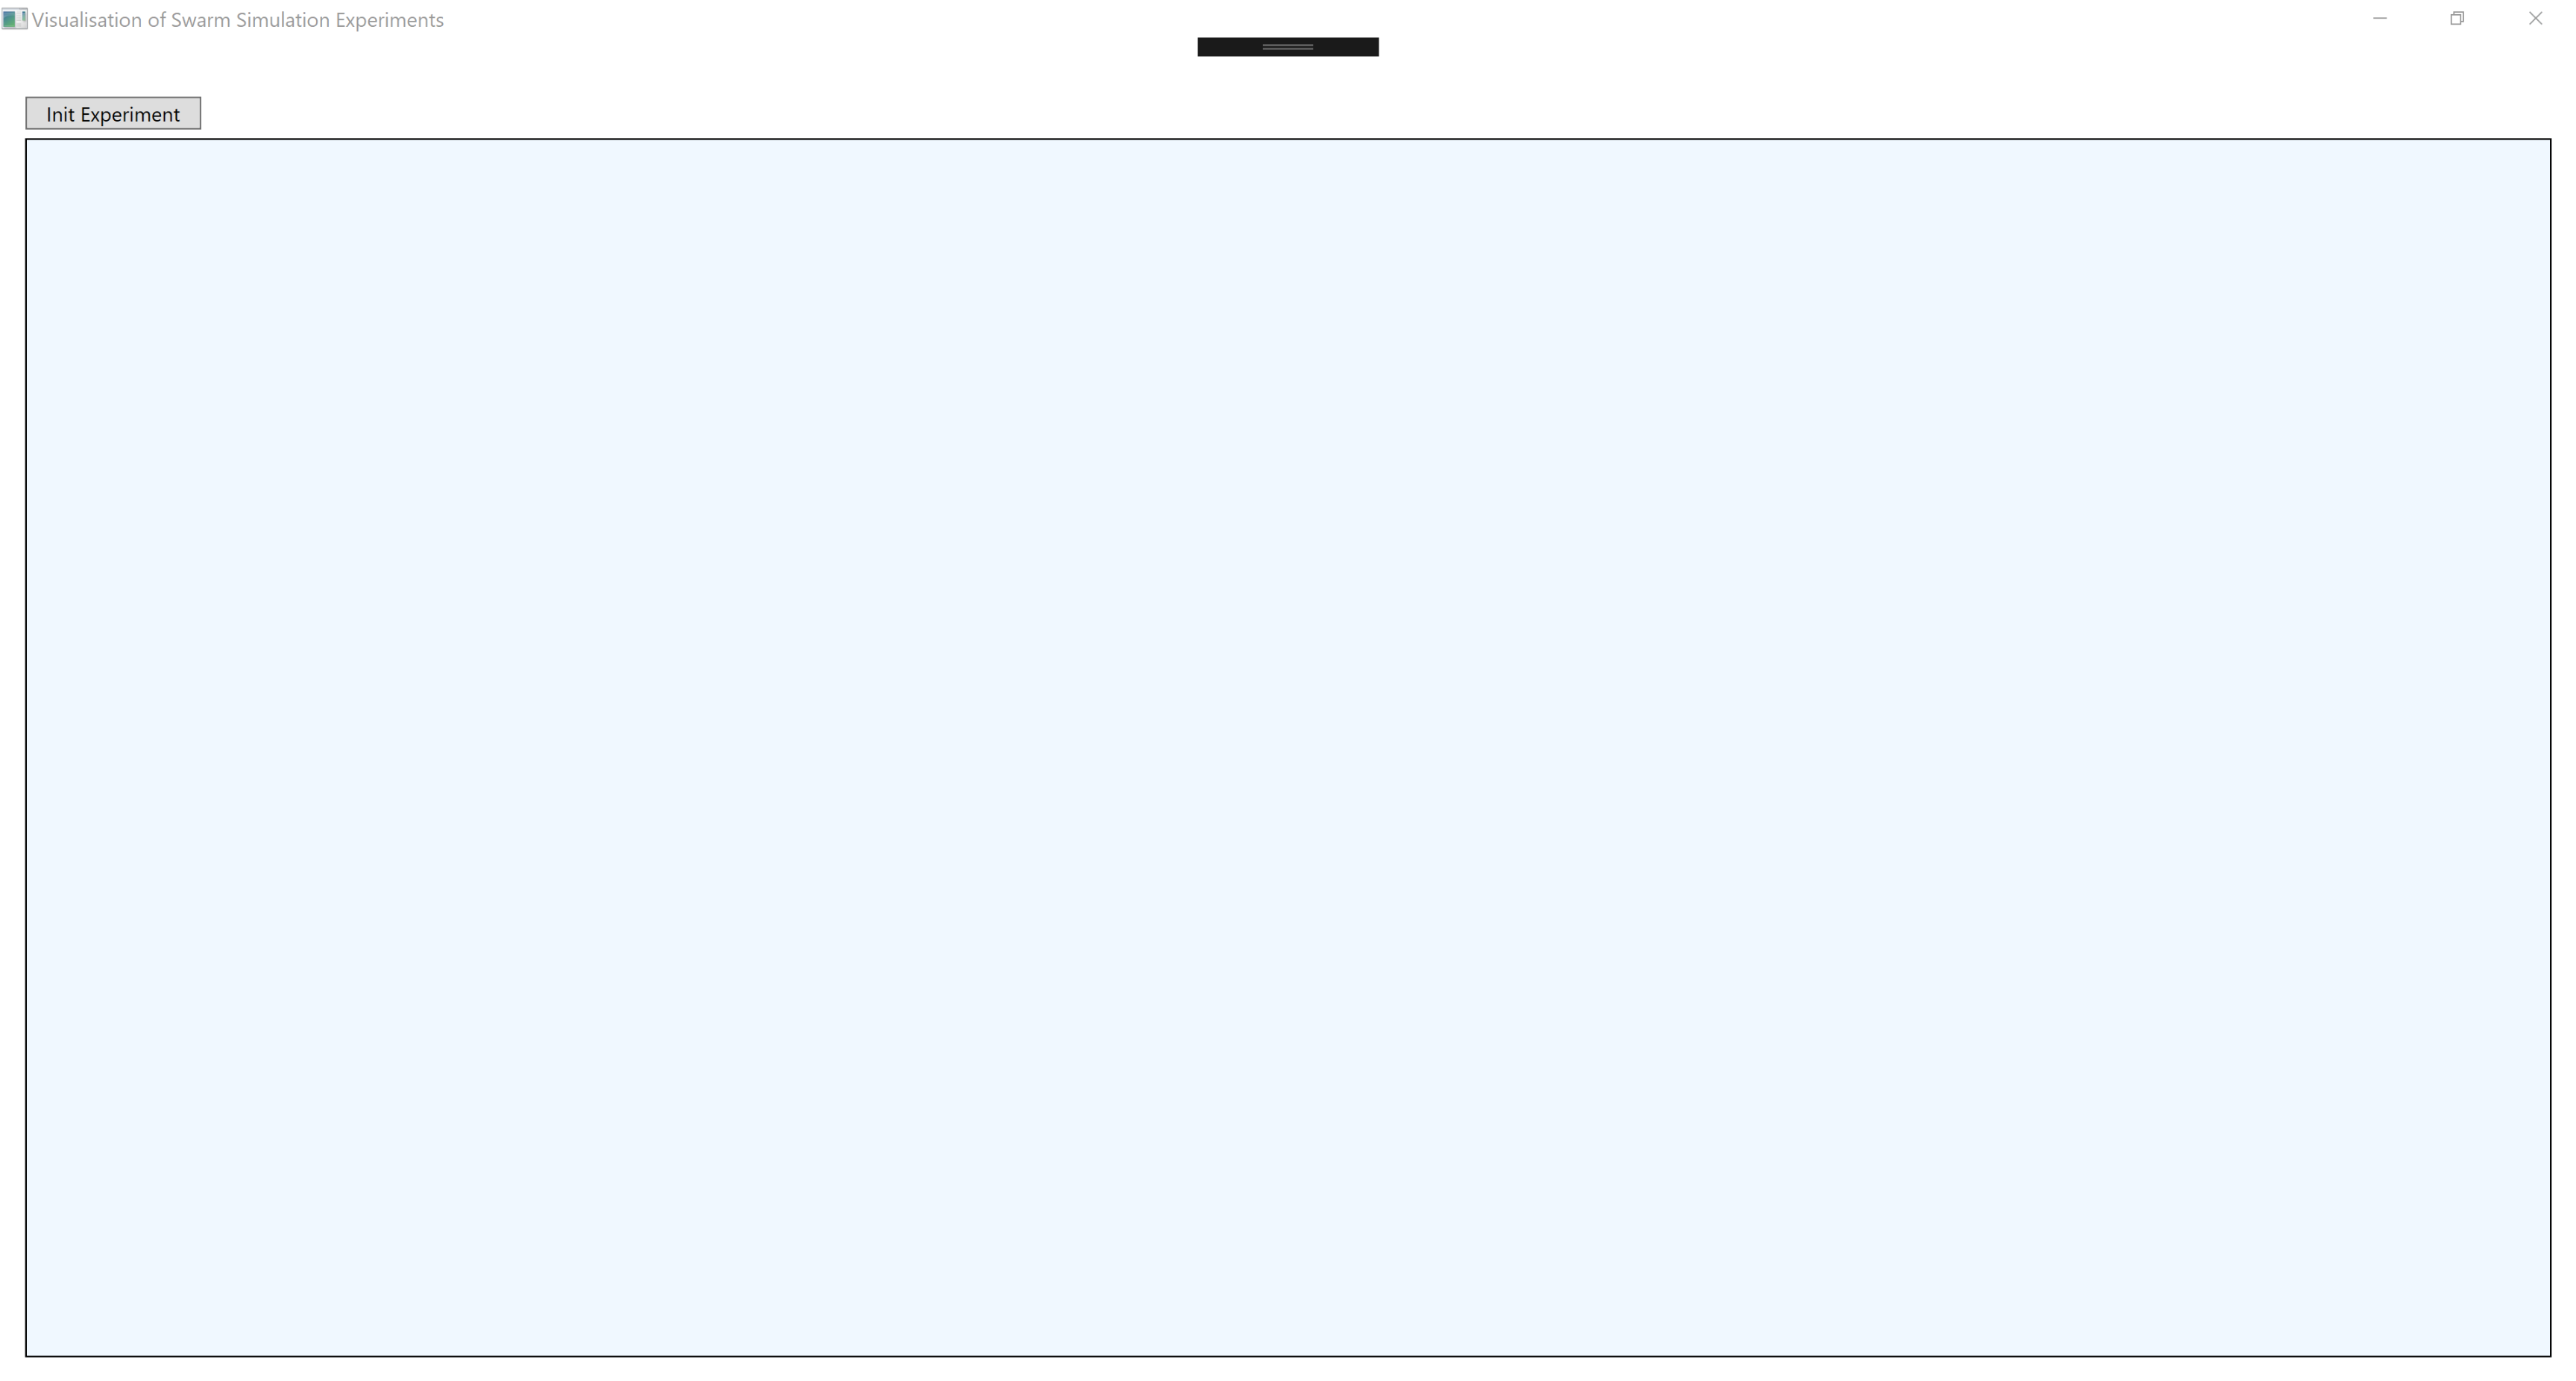
\includegraphics[width=\columnwidth]{img/start.png}
		\caption{GUI - Úvodní obrazovka} 
\end{figure} 
\clearpage
Tlačítkem init začneme přípravu experimentu, v následujícím nastavení vybereme požadovanou mapu a roboty, které si chceme prohlédnout. V \textit{Length of Cycle} můžeme zvolit délku simulace (počet iterací mapy). 
\par
\begin{figure}[h]\centering
	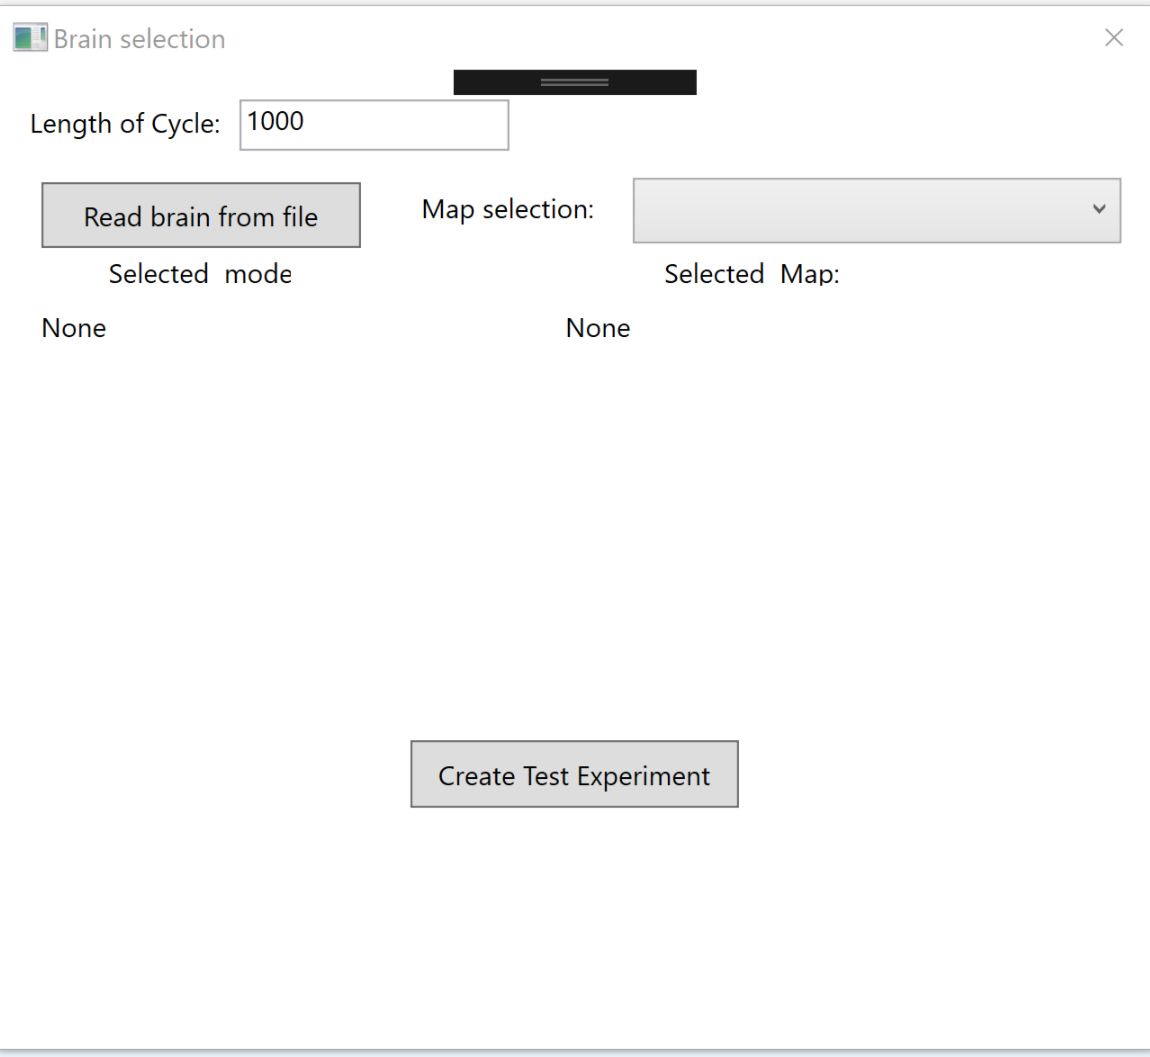
\includegraphics[width=\columnwidth]{img/brain_sel.png}
	\caption{GUI - vytoření experimentu} 
\end{figure} 
\clearpage
Na vybrané mapě můžeme nastavit počty jednotlivých objektů na mapě. Ostatní hodnoty jsou pouze informativní.
\par
\begin{figure}[h]\centering
	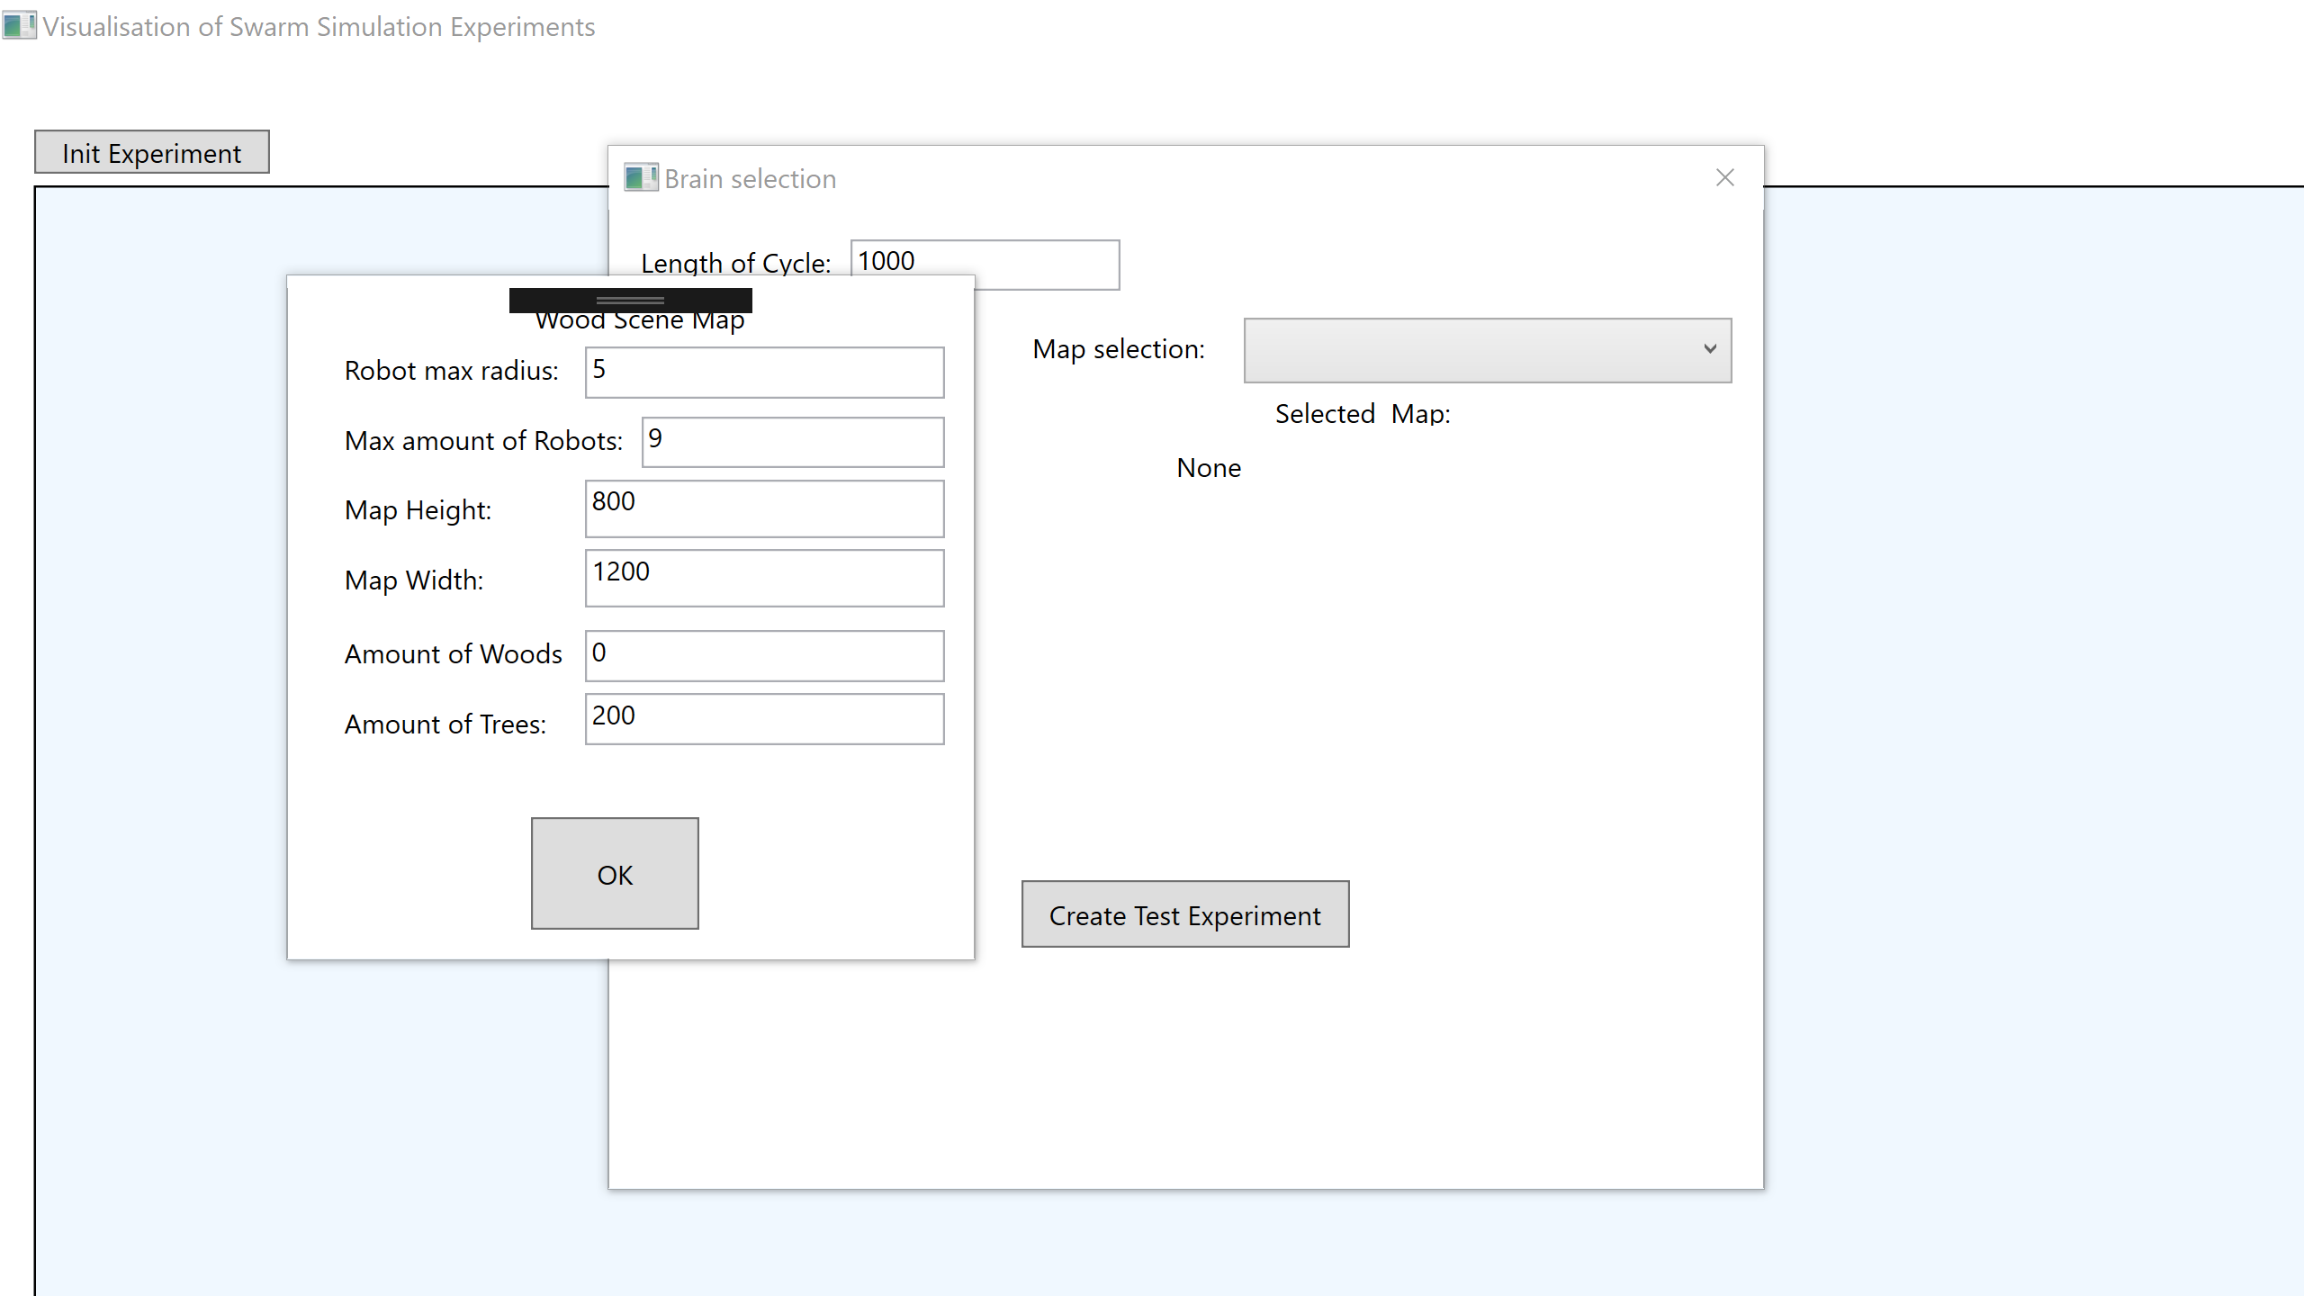
\includegraphics[width=\columnwidth]{img/map_sel.png}
	\caption{GUI - nastavení mapy} 
\end{figure} 
\clearpage
Dále je potřeba zvolit roboty a propojit je s robotickým mozkem (neuronovou sítí). K čemuž slouží tlačítko \textit{Read brain from file}. 
\par
\begin{figure}[h]\centering
	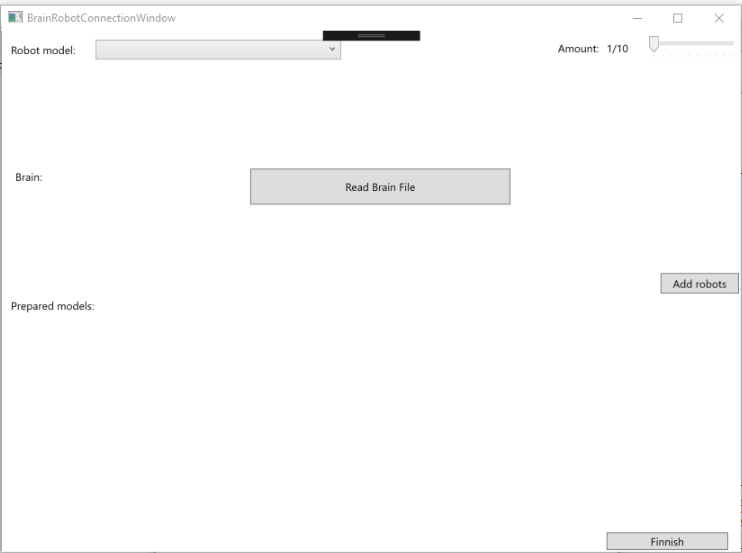
\includegraphics[width=\columnwidth]{img/brain_con.png}
	\caption{GUI - přidání robotů s ovládáním } 
\end{figure} 
V tomto okně můžeme nastavit druh robota \textit{Robol model} a jejich počet v mapě. Tyto zvolené roboty musíme spojit s kompatibilním chování pomocí tlačítka \textit{Read Brain File}, které otevře okno pro výběr soubor a je potřeba zvolit soubor s jedním serializovaným mozkem. Pokud je mozek kompatibilní k robotovi, objeví se jeho detaily po nápisem \textit{Brain}. Pak jen stačí přidat je do simulace tlačítkem \textit{Add robots} (pozor na limit počtu robotů v simulaci je kontrolován až na konci propojování).
\clearpage
Vyplněné okno pro projování vypadá následovně. Projování s roboty je potřeba potvrdit tlačítek \textit{Finnish}.
\begin{figure}[h]\centering
	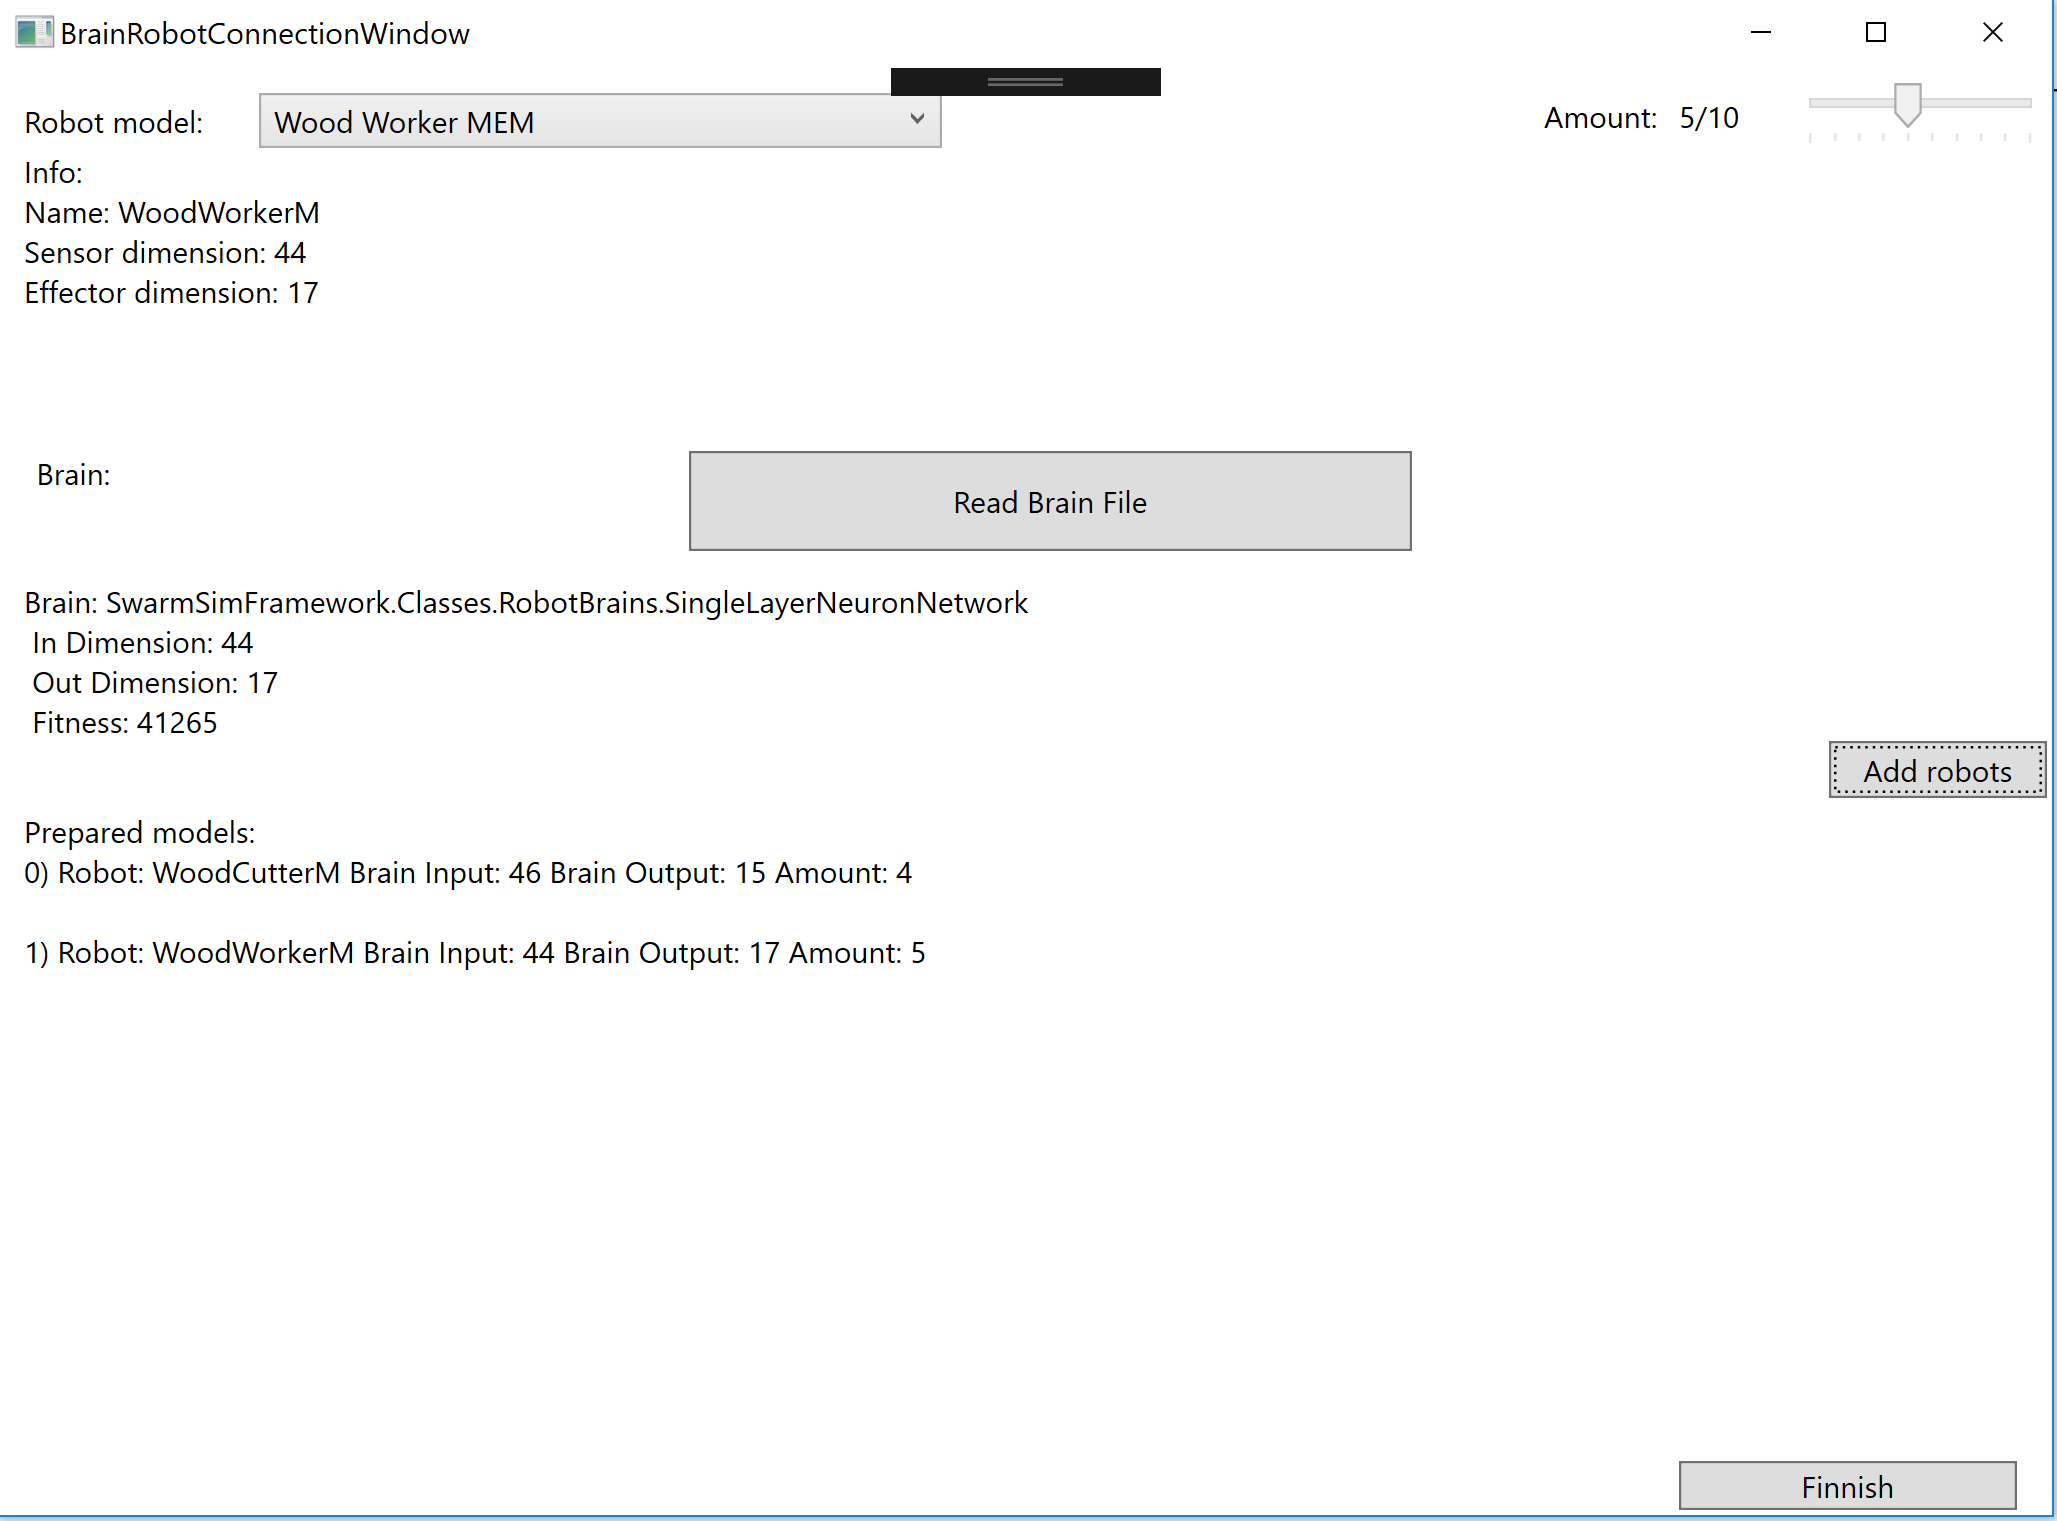
\includegraphics[width=\columnwidth]{img/brain_con_full.png}
	\caption{GUI - vyplěné přidání robotů s ovládáním } 
\end{figure}
\clearpage
Nyní je vše připraveno pro pozorování simulaci, po stisknutí tlačítka \textit{Create Test Experiment} se inicializuje námi specifikovaný experiment. V levém horním rohu se nácházejí ovládací tlačítka \textit{Run} spustí simulaci, \textit{Pause} pozastaví simulaci, \textit{Stop} ji úplně zastaví. 
\begin{figure}[h]\centering
	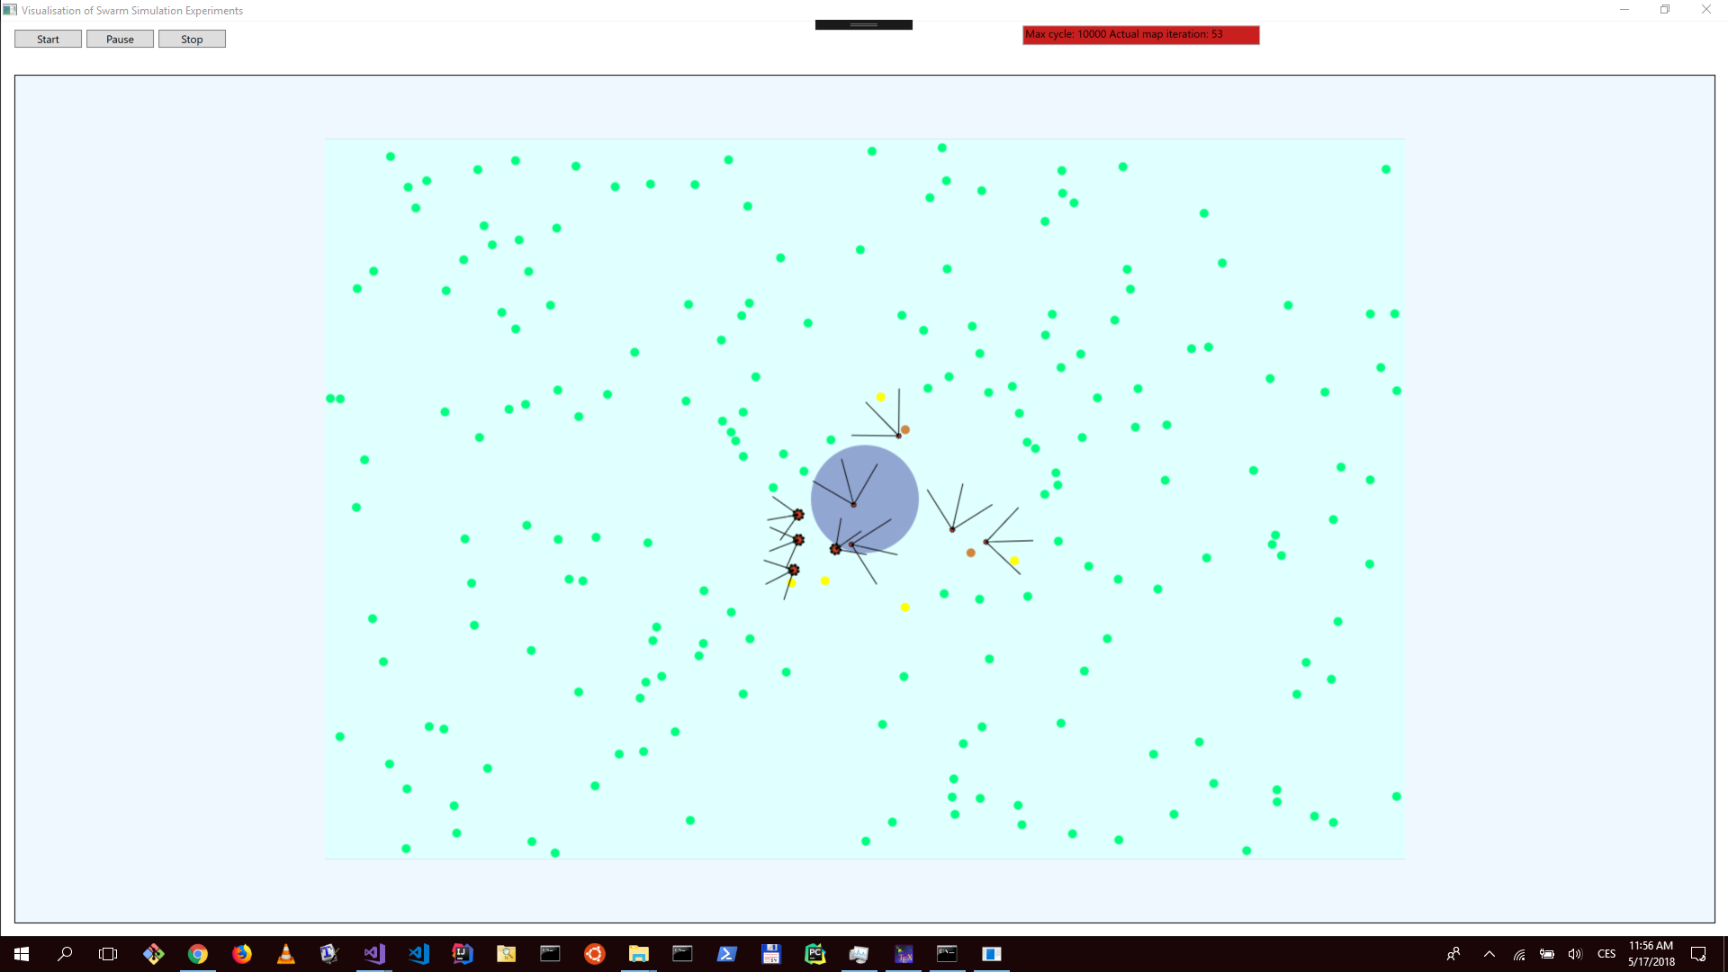
\includegraphics[width=\columnwidth]{img/experiment_run.png}
	\caption{GUI - začátek experimentu } 
\end{figure}
\clearpage 
Při pozastavené simulaci si můžeme pravým kliknutím na robota o něm zobrazit podrobné údaje.
\begin{figure}[h]\centering
	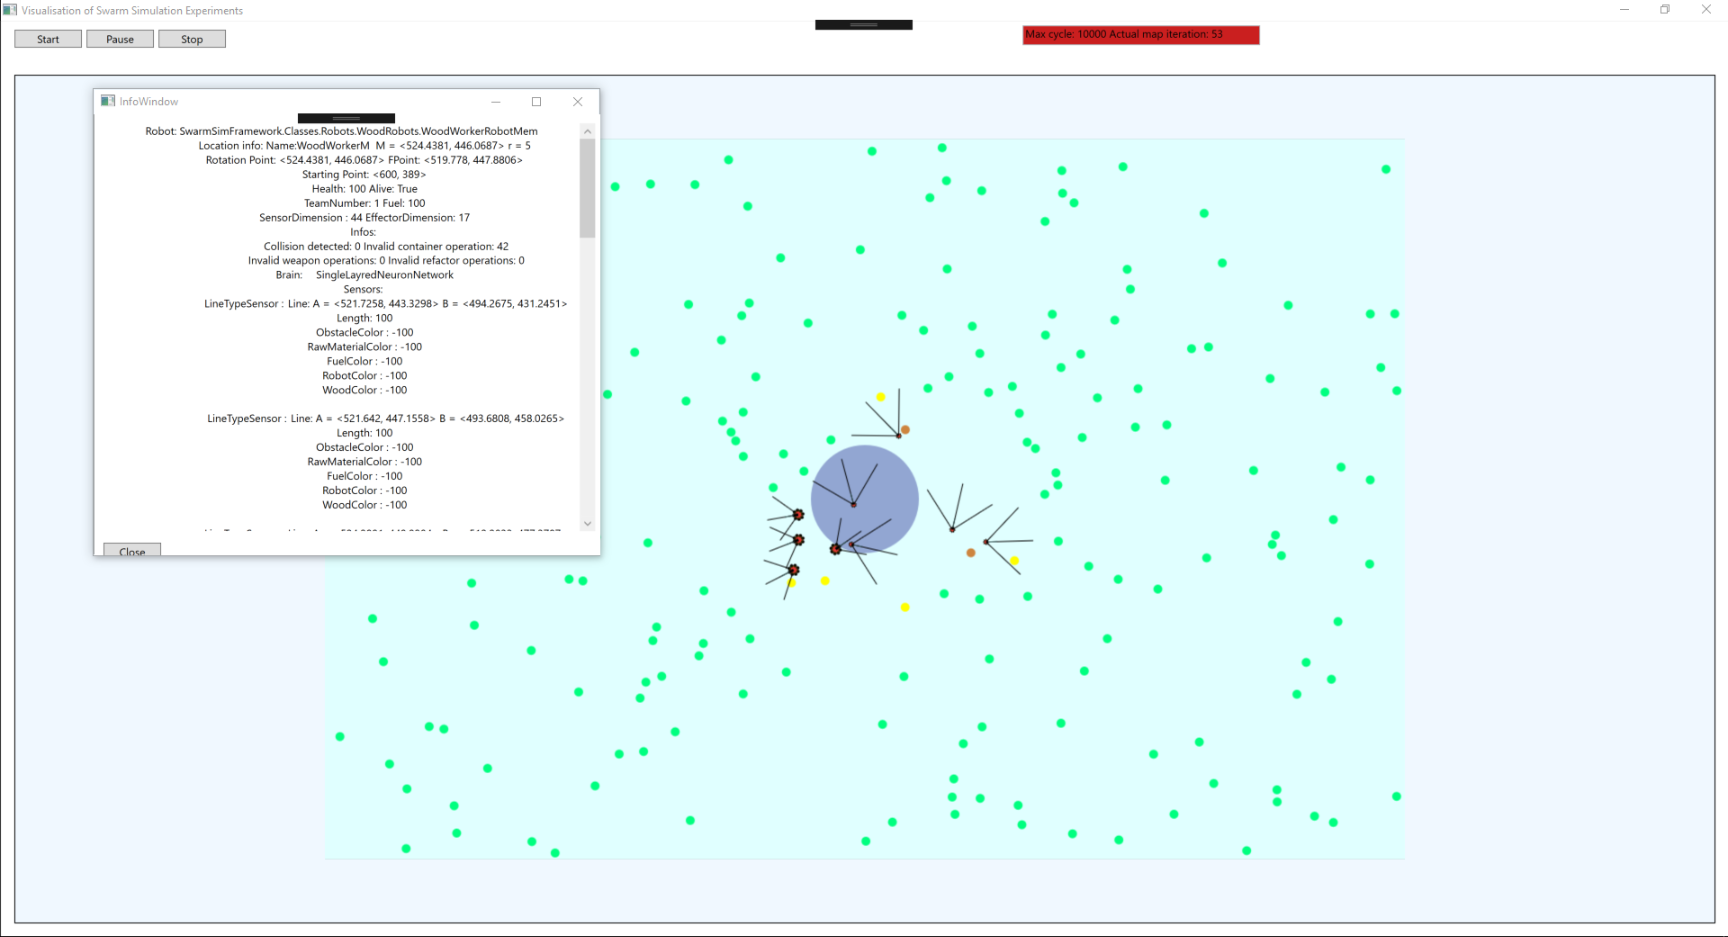
\includegraphics[width=\columnwidth]{img/info_click.png}
	\caption{GUI - dodatečné informace} 
\end{figure}
\clearpage 
\clearpage
\section{Programátorská dokumentace}
\subsection{Úvod:}
Map je centrální třídou projektu, zajištuje vlastní průběh simulace. Uchovává jednotlivé entity (roboty,  překážky, palivo, minerály), volá vyhodnocení akcí pro aktivní entity(roboty) včetně počítání kolizí a interakcí s mapou(přesuny pasivních entit, vysátí paliva, atd..). Potomci třídy entita reprezentuje objekt v mapě, všechny jsou  odděny od stejného předka. V celém projektu se vyskytují 2 tvary entit, konkrétně se jedná o úsečku(sensory, efektory) dále o kruh(roboti, překážky, minerály). Robot zastává pozici aktivní entity pohybující se na mapě a interagující s ostatními entitami. Ke komunikaci, pohybu a změnám se v mapě používá robot efektory a sensory. Sensory se používají ke čtení informací z mapy, tedy vrací vektor čísel representující rozdílné vlasnosti mapy(vzdálenostní sensory, rádiové etc.), zatímco efektory mají opačný účel, tedy ovlivňovat mapu a entity a příjímají vektor čísel jako nastavení konkrétního efektory. Sensor a Efektor jsou implementací rozhraní ISensor a IEffector(viz. další kapitola). Pro simulování chování robotů slouží tzv. "mozek", v programu IRobotBrain, který má za úkol z vektoru ze všech sensorů vytvořit vektor pro všechny efektory a tímto způsobem řídit chování robota. \par
Vývin jednotlivých mozků je řízen přes experiment, což je pojem implementován v projektu různými způsoby dle požadavků uživatele. (MultiThreadExperiment, Experiment). Jejich společným cílem je nastavení parametrů dané mapy(počet překážek, druhy robotů..), iterace přes simulační kroky, průběh generací mozků, změnu mozků(differenciální evoluce, mutace..). Následně ukládání mezivýsledků a zobrazování postupu daného experimentu. 
\subsection{Hlavní třídy:}
\begin{itemize}
	\item Sensors - sensory, které čtou data z  mapy 
	\item Efektory - interakce s mapou a ostatními entitami
	\item Entities - Reprezentace jednotlivých entit, které se vyskytují na mapě. Všechny entity jsou odděděny od abstraktního předka \textbf{Entity}. 
	\item Experiments - jednotlivé parciální evoluce pro řešení daného úkolu, které počítají s visualizací
	\item Map - Reprezentace 2D prostředí, kde se všechny entity pohybují, zajištuje kontrolu kolizí a celý průběh simulací. Také obsahují jednotlivé části evolučních algoritmů pro vícevláknový běh evolučních strategií. 
	\item MultiThreadExperiment - jednotlivé parciální experimenty, optimalizované pro  běh na více vláknech bez GUI. 
	\item RobotBrains - Reprezentace jednotlivých mozků implementující interface IRobotBrain
	\item Robots - konkrétní reprezentace robotů 
\end{itemize}
\newpage
\subsection{Map} 
Reprezentace 2D prostředí simulace. Mapa je daná obdélníkem o dané velikosti při konstrukci. Běhemi konstrukce také dostává všechny entity ve výchozích pozicích, co se budou v prostředí vyskytovat, také vytvoří jejich klony, aby později bylo možné vrátit mapu do  počátečního stavu. Existují 4 základní typy entit v mapě. Jedná se o  Robots - aktivní entity(IRobotEntity), na které je při každém kroku mapy, zavolána nejdříve PrepareMove() a dále Move() v náhodném pořadí, aby žádný robot nebyl upřednostěn. PasiveEntities pasivní entity, buď překážky nebo jiné nezpracované materiály. (CircleEntity), FuelEntities- palivo vyskytující se v mapě, pokud je spotřebováno je odebráno z tohoto seznamu. Jako poslední RadioEntities, což je vrstva rádiových signálů, které se počítají jen pro speciální kolize. \par 
MakeStep()  je metoda provádějící jeden krok simulace. 
Mapa charakterizují 4 krajní body A,B,C,D, také aktuální cyklus(počet zavolaných MakeStep()).
\begin{itemize}
	\item Kolize: 
	\begin{itemize}
		\item Pro CircleEntity vrací bool, zda s něčím koliduje. 
		\item pro LineEntity vrací průsečík s nejbližším objektem mimo fuel na něj  je speciální metoda. 
		\item pro CircleEntity reprezentující rádiový sensor, vrací slovní všech průsečíku s rádiovými  signály. 
		\item pro  CircleEntity existuje metoda CollisionColor, která vrací všechny průsečíky v dosahu CircleEntity.
	\end{itemize} 
	\item SceneMap - konkrétní mapy pro jednotlivé experimenty MineralScene, WoodScene, CompetitiveScene
	\item Intersection - struktura pro  jednotlivé druhy průsečíků z kolizí
\end{itemize} 
\newpage
\subsection{Rozhraní}
\begin{itemize}
	\item IEffector
	- definuje efektor, který ovlivňuje pohyb a interakce robota s mapou. \\
	- k jeho použití slouží funkce Effect(float[] settings, RobotEntity robot, Map.map map). Settings určuje, jakým způsobem ovlivňuje robota a danou mapu. Před 1. použitím efektoru je nutné robota připojit, pomocí funkce ConnectToRobot(RobotEntity robot), která nastaví normalizační funkce(= rozsahy a transformace hodnot přicházející od robota) 
	\item ISensor 
	- definuje sensor, který čte prostředí simulace \\
	- k jeho použití slouží funkce float[] Count(RobotEntity robot, Map.Map map), která dle pozice robota vrátí informace, přečtené z mapy. Druh informací se liší konkrétními implementacemi. Před první použitím jiného robota je nutné analogicky jako u efektoru robot připojit pomocí funkce ConnectToRobot(RobotEntity robot).
	\item IRobotBrain - definuje mozek robot, tzn. jeho chování. Slouží k transformaci vektoru přicházejího ze sensorů na vektor vstupující do efektorů. K tomuto účelu slouží fce float[] Decide(float[] readValues). Dále každý mozek lze ohodnotit hodnotou Fitness, dle jeho úspěšnosti v simulaci. Každý mozek má vstupní a výstupní velikost (IoDimension),  rozsahy hodnot pro výstup a vstup (InOutBounds), převodní funkci z interní hodnot počítání vstupu na hodnoty výstupní (Activation func), umí vytvořit svou čistou kopii (GetCleanCopy), případně se (de)serializovat (z)do json formátu. 
	\item IExperiment - definuje průběh experimentu, ale je vhodný pro visualizační řešení. Obsahuje mapu na které je simulace prováděná. Každé volání MakeStep() provede nejmenší krok simulaci(jeden pohyb každé entity). Experiment musí být inicializován metodou Init(). Pokud experiment dosáhl svého cíle, FinnishedGeneration je nastaven na true. 
\end{itemize}
\newpage
\subsection{Efektory a sensory:} 
\subsubsection{Effectors:}
- obsahuje konkrétní implementace efektorů, všechny třídy jsou odděděny od IEffector. Jedná se o efektory určené pro vzorové scénáře. Mohou být rozšířené skrz IEffector. \\
\begin{itemize}
	\item MineralRefactor - slouží k přeměně minerálů (RawMaterialEnitity) na palivo. Refaktoruje entitu na vrcholu kontejneru robota. 
	\item Picker - implementovaný jako LineEntity, slouží ke zvedání entit, které se protínají s jeho úsečkou. Dále umí na úsečku pokládat entity z vrcholu zásobníku. 
	\item RadioTransmitter - umí vysílat rádiové  různé rádiové signály dle nastavení Effect
	\item TwoWheelMotor - pohybuje s robotem, dle nastavení rychlostí koleček. Fyzikální model, lze najít, zde  \url{http://rossum.sourceforge.net/papers/DiffSteer/DiffSteer.html}. 
	\item Weapon - dle nastavení může působit poškození robotům, protínající úsečku jeho působnosti.(LineEntity) 
	\item WoodRefactor - slouží k přeměně RawMaterialEnitity, pokud protínají úsečku jeho působnosti(LineEnitity), přímo na mapě. Přeměněná entita tedy nemusí být v kontejneru.
\end{itemize}
\subsubsection{Sensors:}
- obsahuje konkrétní implementace sensorů, všechny třídy jsou  odděděny od ISensor. Jedná se o sensory pro vzorové scénáře. Mohou být rozšířené skrz ISensor.
\begin{itemize}
	\item FuelLInSensor - Sensor, který vrací vzdálenost od Fuel, pokud úsečka (LineEntity) nějaké na mapě protíná.
	\item LineTypeSensor - Sensor, který vrací vzdálenost od libovolné Enity(mimo fuel, rádiové signály) a jeho typ(EntityColor). Pokud nějakou na mapě protíná(LineEntity). 
	\item LocatorSensor - Sensor, který vrací aktuální polohu robota a jeho orientaci vzhledem ke středu robota. 
	\item MemoryStick - Sensor a Efektor v jednom, slouží k zapisování float do paměti. Pokud k němu přistupuji jako k sensoru vrací uložené hodnoty, pokud jako k effektoru, tak ukládá zapisované hodnoty. 
	\item RadioSensor - Sensor, který vrací přečtené signály z okolí a průměr z jejich umístění. Implementován jako CircleEntity. 
	\item TouchSensor - Sensor, který vrací jen binární hodnotu, zda protíná nějakou entitu nebo nikoliv. Implementován jako CircleEntity. 
	\item TypeCircleSensor - Sensor, který vrací binární hodnotu pro každý druh entity(Entity Color), která říká, zda je daná entita v jeho okolí či nikoliv.
\end{itemize}

\subsection{Entity}
\subsubsection{abstract class Entity}
Reprezentuje společného předka a implementuje zakladní společné vlastnosti a metody pro všechna entity pasivní i nepasivní. Definuje vlastnost Color určující účel entit v mapě. 
\begin{itemize}
	\item ObstacleColor
	\item RawMaterialColor
	\item FuelColor
	\item RobotColor
	\item WoodColor 
\end{itemize}
Dále jsou od Entity odděleny základní dva tvary entit abstraktní třídy CircleEntity a LineEntity, které přidávají konkrétní implementace pohybových funkcí a 	přidávají některé další vlastnosti. 

\subsubsection{CircleEntity:}
Přepisuje metody MoveTo, RotateRadians pro  pohybování kruhu. Přidává vhodné konstruktory. \\ 
\subsubsection{LineEntity:}
Přepisuje metody MoveTo, RotateRadians pro pohybování úsečkou. Přidává vhodné konstruktory. \\ 
\newpage
\subsubsection{RobotEntity}
Potomek třídy CircleEntity, který tvoří základ pro jednotlivé roboty. Uchovává konkrétní instance efektorů a sensorů, zajišťuje komunikaci mezi nimi a mozkem(i převody jednotlivých rozsahů. Přidává další vlastnosti jako životy, množství paliva, číslo týmu, kontejner(možnost přesouvat a uchovávat ostatní instance třídy Entity). \\ 
\textbf{Některé důležitější metody:} 
\begin{itemize}
	\item List<CircleEntity> ContainerList() - robot může mít kontejner na CircleEntities, dané kapacity při vytváření robota, tata metody vratí celý jeho obsah
	\item PrepareMove(Map.Map map) - na dané mapě provede výpočet na všech sensorech a dané hodnoty předá mozku na zpracování, uloží vstup pro efektory z mozku. 
	\item Move(Map.Map map) - spustí všechny efektory na základě vektoru vypočítaného v předchozí metodě. 
	\item Metody spojené s kontejnerem - PushContainer, PopContainer, PeekContainer
\end{itemize}
\subsubsection{Ostatní CircleEntity: }
\begin{itemize}
	\item FuelEntity - pasivní entita, která reprezentuje nádobu s palivem
	\item ObstacleEntity - pasivní entita, reprezentující překážky
	\item  RadioEntity  - pasivní entita, reprezentující rádiový signál s danou informací 
	\item  RawMaterialEntity - pasivní entita, reprezentující nezpracovaný materiál (strom, minerál) 
	\item  WoodEntity - pasivní entita, reprezentující zpracovaný materiál vytěžené dřevo
\end{itemize}
\newpage \label{key}
\subsection{MultiThread}
Základem MT experimentů je bstract class MultiThreadExperiment<T>, kde T je potomek IRobotBrain druh mozku, který vyvíjí. Tato třída obsahuje základní nastavení evoluce. (velikost populace, jméno, počet iterací atd..). Před spuštěním fce Run() je potřeba připravit Mapu a modely mozků, robotů pomocí přetížení abstraktní metody Init(). Funkce Run() - pouští jednotlivé členy aktuální populace každou na jiném vlákně, jejich ohodnocení je implementována pomocí abstraktní metody CountFitness(map). Takto pokračuje napříč všemi generacemi až do poslední. Během běhu serializuje nejlepší mozky, graf(,pokud PC obsahuje GNUplot, tak i vykresluje), všechny mozky(ve zvolených generacích) . \\
Složky Mineral Scene a WoodScene obsahují vzorové příklady experimentů pro scénáře WoodScene a MineralScene.
\subsection{RobotBrains} 
Třídy definující chování robotů. Základním principem je funkce, která přijme vektor float hodnot a  z něj vytvoří jiný vektor float. Vstupní hodnoty předává robot ze sensorů a výstupní hodnoty jsou použity pro nastavení efektorů. Projekt obsahuje 3 základní mozky:
\begin{itemize}
	\item FixedBrain - mozek, který ignoruje vstup a vrací daný výstup 
	\item Perceptron - základní prvek neuronových sítí (vážený součet)  lib. vstup a jeden výstup
	\item SingleLayerNeuronNetwork - neuronová síť tvořená z perceptronů.
\end{itemize}

Pro SingleLayredNetwork je připravený evoluční algoritmus Differenciální evoluce, definovaná dle  \url{https://en.wikipedia.org/wiki/Differential_evolution}.

\subsection{Externí knihovny, NuGet}
\begin{itemize}
	\item Intersection2D - implementace jednoduchých průsečíků mezi kruhem, přímkou 
	\item MathNet.Numerics - pokročilé matematické funkce, používané v evolučních  algoritmech, normální rozdělení apod.
	\item Newtonsoft.Json - serializace do jsonu
	\item System.Numerics - reprezentace Vektorú
	
\end{itemize} 
\subsection{Support třídy} 
\begin{itemize}
	\item ActivationFuncs - funkce pro převod hodnot ze sensorů do efektorů
	\item GNUPlot - knihovna pro ovládání programu GNUPLOT 
	\item RandomNumber  - statická třída pro volání náhodných tříd
	\item SupportClasses - ostatní pomocné třídy
	
\end{itemize}

\newpage
\section{Ostatní projekty:}
\subsection{SwarmSimVisu:}
Motivací pro tento projekt je sledování, ladění chyb a v neposlední řadě také pozování vyvinutých mozků a chování dokončených experimentů. Pro debugovací účely umí pouštět jednotlivé potomky třídy Experiment, kde lze sledovat průběh experimentů. Na kontrolu vyvinutých mozků je k dispozici Experiment "Testing Brain", kde mohu připravit experiment simulující průběh mapy, kde se pohybují mnou zvolené entity s nahraným serializovaným mozkem. Vykreslování probíhá přes třídu MapCanvas, kde je použita externí třída D2dControl.D2dControl. Centrální třídou je MainWindow, které spouští jednotlivé Experimenty. Instance třídy InfoWindow slouží pro krátké informativní zprávy. Pro sestavení vlastního "Testing Brain" experimentu jsou k dispozici dvě okna BrainSelectionWindow(nastavení globální parametrů simulace), BrainRobotConnectionWindow(připravení mozků a robotů). 
\subsection{InterSection2d:}
Jedná se  jednoduché průsečíky kruhu, přímek, úseček v 2D prostoru. Projekt cílí na rychlost, neboť se jedná o nejvíce volané třídy z celého projektu.
\par
\end{document}